\documentclass[12pt,a4paper]{article}
\usepackage[utf8]{vietnam}
\usepackage{amsmath,amssymb}
\usepackage{geometry}
\geometry{top=1.5cm,bottom=1.2cm,left=1.4cm,right=1.4cm,headheight=28pt,headsep=12pt,footskip=18pt}
\usepackage{tikz}
\usepackage{xcolor}
\usepackage{enumerate}
\usepackage{graphicx}
\usepackage[version=4]{mhchem}
\usepackage{fancyhdr}
\usepackage{ex_test}

\renewcommand{\baselinestretch}{0.96}
\setlength{\parskip}{0pt}

\definecolor{hfRed}{RGB}{211,47,47}
\definecolor{hfGreen}{RGB}{139,195,144}

\pagestyle{fancy}
\fancyhf{}
\fancyhead[L]{\small\itshape\color{hfRed} Tài liệu lưu hành nội bộ}
\fancyhead[R]{\small\itshape\color{hfRed} Thầy \textbf{TRẦN VĂN THẠNH} - 0777.470.803}
\renewcommand{\headrulewidth}{0.8pt}
\renewcommand{\headrule}{\hbox to\headwidth{\color{hfGreen}\leaders\hrule height \headrulewidth\hfill}}

\fancyfoot[L]{\small\itshape\color{hfRed} CS1: 6/15 Nguyễn Hoàng, P. Kim Long, TP Huế \quad|\quad CS2: 24 Đặng Thái Thân, TP Huế}
\fancyfoot[R]{\small\bfseries\color{hfRed} Trang \thepage}
\renewcommand{\footrulewidth}{0.8pt}
\renewcommand{\footrule}{\hbox to\headwidth{\color{hfGreen}\leaders\hrule height \footrulewidth\hfill}}

\fancypagestyle{firstpage}{
  \fancyhf{}
  \renewcommand{\headrulewidth}{0pt}
  \fancyfoot[L]{\small\itshape\color{hfRed} CS1: 6/15 Nguyễn Hoàng, P. Kim Long, TP Huế \quad|\quad CS2: 24 Đặng Thái Thân, TP Huế}
  \fancyfoot[R]{\small\bfseries\color{hfRed} Trang \thepage}
  \renewcommand{\footrulewidth}{0.8pt}
  \renewcommand{\footrule}{\hbox to\headwidth{\color{hfGreen}\leaders\hrule height \footrulewidth\hfill}}
}

\begin{document}
\thispagestyle{firstpage}

\noindent
\begin{minipage}[t]{0.44\textwidth}
	\centering\fontsize{10pt}{12pt}\selectfont
	\textbf{SỞ GIÁO DỤC VÀ ĐÀO TẠO THỪA THIÊN HUẾ}\\
	\textbf{ĐỀ CHÍNH THỨC}\\
	\textit{(Đề thi có 04 trang)}
\end{minipage}\hfill
\begin{minipage}[t]{0.54\textwidth}
	\centering\fontsize{10.5pt}{13pt}\selectfont
	\textbf{ĐỀ KIỂM TRA ĐỊNH KỲ CHƯƠNG 6}\\
	\textbf{(HỢP CHẤT CARBONYL - CARBOXYLIC ACID)}\\
	\textbf{MÔN: HOÁ HỌC - LỚP 11}\\
	\textit{Thời gian làm bài: 50 phút, không kể thời gian phát đề}
	
	\smallskip
	\fbox{\textbf{MÃ ĐỀ: 116}}
\end{minipage}

\smallskip
\noindent\hrulefill
\smallskip

\noindent\textbf{Họ, tên thí sinh:} \dotfill\ \textbf{Lớp:} \dotfill\ \textbf{Số báo danh:} \dotfill

\smallskip
\noindent\textit{(Cho biết nguyên tử khối: H = 1; C = 12; N = 14; O = 16; Na = 23; Mg = 24; Al = 27; P = 31; S = 32; Cl = 35,5; K = 39; Ca = 40; Cr = 52; Mn = 55; Fe = 56; Cu = 64; Zn = 65; Br = 80; Ag = 108; Ba = 137.)}

\smallskip
\noindent\textbf{\large PHẦN I. Câu trắc nghiệm nhiều phương án lựa chọn.}
\textit{Thí sinh trả lời từ câu 1 đến câu 18. Mỗi câu hỏi thí sinh chỉ chọn một phương án.}
\vspace{0.2cm}

\begin{ex}
Công thức tổng quát của aldehyde no, đơn chức, mạch hở có thể là công thức nào trong số các công thức sau:
\choice
{\ce{C_xH_{2x+1}CHO} ($x$ nguyên, không âm) hoặc \ce{C_xH_{2x}O} ($x$ nguyên dương)}
{\ce{C_xH_{2x}O} ($x$ nguyên dương)}
{\ce{C_xH_{2x+2}CHO} ($x$ nguyên, không âm)}
{\ce{C_xH_yCHO}}
\end{ex}

\begin{ex}
Chất nào sau đây là formic aldehyde?
\choice
{\ce{HCHO}}
{\ce{CH3CHO}}
{\ce{C2H5OH}}
{\ce{C2H6}}
\end{ex}

\begin{ex}
Khử \ce{HCHO} bằng \ce{LiAlH4} thu được sản phẩm là
\choice
{\ce{CH3CHOHCH3}}
{\ce{CH3OH}}
{\ce{CH3COOCH3}}
{\ce{CH3COOH}}
\end{ex}

\begin{ex}
Khử \ce{CH3COCH3} bằng \ce{LiAlH4} thu được sản phẩm là
\choice
{\ce{CH3COOCH3}}
{\ce{CH3CHOHCH3}}
{\ce{CH3COOH}}
{\ce{CH3CH2OH}}
\end{ex}

\begin{ex}
\textbf{[KNTT - SBT]} Ba chất A, B, C có nhiệt độ sôi được biểu thị như hình sau:
\begin{center}
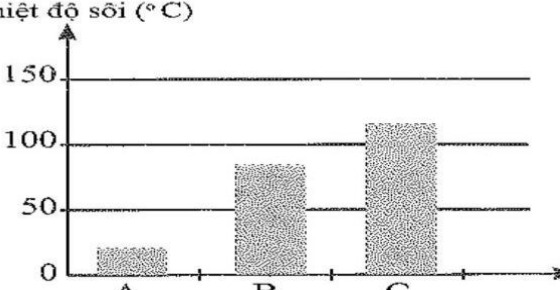
\includegraphics[width=0.38\linewidth]{images_crop_hoa11_de16/boiling_point_bar_chart.png}
\end{center}
Các chất A, B, C lần lượt là
\choice
{ethanol, acetaldehyde, acetic acid}
{acetaldehyde, ethanol, acetic acid}
{acetaldehyde, acetic acid, ethanol}
{acetic acid, acetaldehyde, ethanol}
\end{ex}

\begin{ex}
\textbf{[KNTT - SBT]} Nhận xét nào sau đây \textbf{không} đúng?
\choice
{Aldehyde vừa có tính oxi hoá, vừa có tính khử}
{Chỉ có ketone tham gia phản ứng tạo iodoform}
{Acid và ester no, đơn chức, mạch hở có công thức chung là \ce{C_nH_{2n}O2}}
{Carboxylic acid làm đổi màu giấy quỳ}
\end{ex}

\begin{ex}
\textbf{(SBT - CTST)} Acetaldehyde thể hiện tính oxi hóa trong phản ứng nào sau đây?
\choice
{\ce{CH3CHO + H2 ->[{Ni, t$^\circ$}] CH3CH2OH}}
{\ce{2CH3CHO + 5O2 ->[{t$^\circ$}] 4CO2 + 4H2O}}
{\ce{CH3CHO + Br2 + H2O -> CH3COOH + 2HBr}}
{\ce{CH3CHO + 2Ag(NH3)2OH -> CH3COONH4 + 2Ag + 3NH3 + H2O}}
\end{ex}

\begin{ex}
\textbf{(SBT - CD)} Phát biểu nào sau đây về tính chất của hợp chất carbonyl là \textbf{không} đúng?
\choice
{Aldehyde phản ứng được với nước bromine}
{Ketone không phản ứng được với \ce{Cu(OH)2/OH^-}}
{Aldehyde tác dụng với dung dịch \ce{AgNO3/NH3} tạo ra bạc}
{Trong các hợp chất carbonyl, chỉ aldehyde bị khử bởi \ce{NaBH4}}
\end{ex}

\begin{ex}
\textbf{(SBT - CD)} Số công thức cấu tạo chứa nhóm carboxylic có cùng công thức \ce{C5H10O2} là
\choice
{2}
{3}
{4}
{5}
\end{ex}

\begin{ex}
Cho chuỗi phản ứng: \ce{C2H6O -> X -> acetic acid ->[{+\ce{CH3OH}}] Y}.\\
Công thức cấu tạo của X, Y lần lượt là
\choice
{\ce{CH3CHO}, \ce{CH3CH2COOH}}
{\ce{CH3CHO}, \ce{CH3COOCH3}}
{\ce{CH3CHO}, \ce{CH2(OH)CH2CHO}}
{\ce{CH3CHO}, \ce{HCOOCH2CH3}}
\end{ex}

\begin{ex}
Cho các chất sau: \ce{CH3-CH2-CHO} (1), \ce{CH2=CH-CHO} (2), \ce{(CH3)2CH-CHO} (3), \ce{CH2=CH-CH2-OH} (4). Những chất phản ứng hoàn toàn với lượng dư \ce{H2} (Ni, $t^\circ$) cùng tạo ra một sản phẩm là:
\choice
{(2), (3), (4)}
{(1), (2), (4)}
{(1), (2), (3)}
{(1), (3), (4)}
\end{ex}

\begin{ex}
Đốt cháy hoàn toàn một aldehyde X, thu được số mol \ce{CO2} bằng số mol \ce{H2O}. Nếu cho X tác dụng với lượng dư \ce{AgNO3} trong dung dịch \ce{NH3}, sinh ra số mol Ag gấp bốn lần số mol X đã phản ứng. Công thức của X là
\choice
{\ce{HCHO}}
{\ce{CH3CHO}}
{\ce{(CHO)2}}
{\ce{C2H5CHO}}
\end{ex}

\begin{ex}
Cho X, Y, Z, T là các chất khác nhau trong số 4 chất: \ce{HCOOH}; \ce{CH3COOH}; \ce{HCl}; \ce{C6H5OH}. Giá trị pH của các dung dịch trên cùng nồng độ 0,01M, ở 25$^\circ$C đo được như sau:
\begin{center}
\begin{tabular}{|c|c|c|c|c|}
\hline
\textbf{Chất} & X & Y & Z & T \\ \hline
\textbf{pH} & 6,48 & 3,22 & 2,00 & 3,45 \\ \hline
\end{tabular}
\end{center}
Nhận xét nào sau đây đúng?
\choice
{Y tạo kết tủa trắng với nước bromine}
{X được điều chế trực tiếp từ ethyl alcohol}
{T bị oxi hóa bởi thuốc thử Tollens}
{Z tạo kết tủa trắng với dung dịch \ce{AgNO3}}
\end{ex}

\begin{ex}
Cho X, Y, Z, T là các chất khác nhau trong số 4 chất: \ce{CH3COOH}, \ce{CH3OH}, \ce{CH3CHO}, \ce{HCOOH} và các tính chất được ghi trong bảng sau:
\begin{center}
\begin{tabular}{|c|c|c|c|c|}
\hline
\textbf{Chất} & X & Y & Z & T \\ \hline
\textbf{Nhiệt độ sôi ($^\circ$C)} & 64,7 & 100,8 & 21,0 & 118,0 \\ \hline
\textbf{pH (dung dịch nồng độ 0,001M)} & 7,00 & 3,47 & 7,00 & 3,88 \\ \hline
\end{tabular}
\end{center}
Chuyển hóa nào sau đây \textbf{không} thực hiện được bằng 1 phản ứng trực tiếp?
\choice
{X $\rightarrow$ Y}
{Z $\rightarrow$ T}
{X $\rightarrow$ T}
{Z $\rightarrow$ Y}
\end{ex}

\begin{ex}
X là xitric acid có trong quả chanh có công thức phân tử là \ce{C6H8O7}, thỏa mãn sơ đồ sau:
\begin{center}
\ce{X ->[{+\ce{NaHCO3}}] C6H5O7Na3 ->[{+\ce{Na}\text{ dư}}] C6H4O7Na4}
\end{center}
Biết rằng xitric acid có cấu trúc đối xứng. Khi cho X tác dụng với \ce{CH3OH} (\ce{H2SO4} đặc, $t^\circ$) thì thu được tối đa bao nhiêu ester?
\choice
{6}
{4}
{5}
{3}
\end{ex}

\begin{ex}
Có bao nhiêu đồng phân có công thức phân tử là \ce{C5H10O} bị oxi hóa bởi thuốc thử Tollens?
\choice
{3}
{4}
{5}
{6}
\end{ex}

\begin{ex}
\textbf{(SBT - CTST)} Methyl salicylate trong thuốc giảm đau được điều chế bằng cách cho salicylic acid phản ứng với methanol có \ce{H2SO4} đặc làm xúc tác, đun nóng. Cho 0,1 mol methyl salicylate phản ứng với dung dịch \ce{NaOH} dư. Số mol \ce{NaOH} đã tham gia phản ứng là
\choice
{0,1 mol}
{0,2 mol}
{0,3 mol}
{0,05 mol}
\end{ex}

\begin{ex}
\textbf{(SBT - CD)} Cho một dung dịch chứa 5,76 gam một carboxylic acid X đơn chức, mạch hở tác dụng hết với \ce{CaCO3} thu được 7,28 gam muối carboxylate. Công thức cấu tạo của X là
\choice
{\ce{CH2=CHCOOH}}
{\ce{CH3COOH}}
{\ce{HC#CCOOH}}
{\ce{CH3CH2COOH}}
\end{ex}

\bigskip
\noindent\textbf{\large PHẦN II. Câu trắc nghiệm đúng sai.}
\textit{Thí sinh trả lời từ câu 1 đến câu 4. Trong mỗi ý a), b), c), d) ở mỗi câu, thí sinh chọn đúng hoặc sai.}
\vspace{0.2cm}

\begin{ex}
Thực hiện thí nghiệm nghiên cứu phản ứng oxi hóa aldehyde theo các bước như sau:\\
\textit{Bước 1:} Cho 2-3 mL dung dịch \ce{AgNO3} 2\% vào ống nghiệm đã rửa sạch. Thêm từ từ dung dịch \ce{NH3} 3\% vào và lắc đều cho tới khi kết tủa tan vừa hết. Thêm khoảng 1 mL dung dịch acetaldehyde 10\% vào ống nghiệm, lắc đều.\\
\textit{Bước 2:} Đặt ống nghiệm vào cốc nước nóng (khoảng 60$^\circ$C) rồi để yên. Sau vài phút lấy ống nghiệm ra khỏi cốc.
\choiceTF
{Sau bước 2, thu được lớp bạc trắng xám bám trên thành ống nghiệm}
{Có thể thay dung dịch acetaldehyde bằng dung dịch acetone sẽ cho kết quả tương tự}
{Ở bước 2, có thể hơ nhẹ ống nghiệm trên ngọn lửa đèn cồn rồi để yên}
{Có thể lắc mạnh ống nghiệm để phản ứng xảy ra nhanh hơn}
\end{ex}

\begin{ex}
Trong nhóm carbonyl \ce{C=O}, nguyên tử carbon liên kết với nguyên tử oxygen bằng 1 liên kết $\sigma$ và 1 liên kết $\pi$ tương tự như trong phân tử alkene.
\choiceTF
{Khử aldehyde hay xeton bằng [H] tạo sản phẩm là các ancol cùng bậc}
{Oxi hóa axetaldehyde bằng nước brom tạo ra sản phẩm là acetic acid}
{Aldehyde fomic có khả năng hòa tan \ce{Cu(OH)2} ở nhiệt độ thường, tạo dung dịch màu xanh lam}
{Aldehyde vừa có tính oxi hóa vừa có tính khử}
\end{ex}

\begin{ex}
Menthone có mùi thơm bạc hà sử dụng làm hương liệu mĩ phẩm, nước hoa, được sản xuất từ menthol theo sơ đồ sau:
\begin{center}
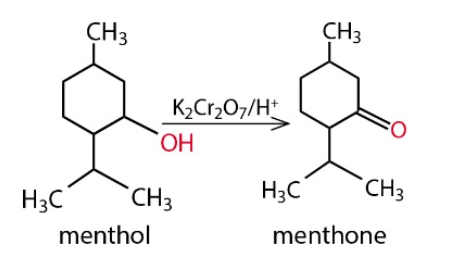
\includegraphics[width=0.45\linewidth]{images_crop_hoa11_de16/menthol_menthone.png}
\end{center}
\choiceTF
{Trong phản ứng trên, menthol bị oxi hóa thành menthone}
{Menthol chứa nhóm chức phenol, menthone chứa nhóm chức carboxyl}
{Công thức đơn giản nhất của menthone là \ce{C10H18O}}
{Có thể chuyển hóa menthone thành menthol bằng tác nhân khử \ce{LiAlH4}}
\end{ex}

\begin{ex}
Nghiên cứu phản ứng ester hóa – điều chế ethyl acetate.\\
Điều chế ethyl acetate trong phòng thí nghiệm được tiến hành như sau:
\begin{itemize}
  \item Cho khoảng 2 ml ethanol và 2 ml acetic acid tuyệt đối vào ống nghiệm, lắc đều hỗn hợp.
  \item Thêm khoảng 1 ml dung dịch \ce{H2SO4} đặc, lắc nhẹ để các chất trộn đều với nhau.
  \item Kẹp ống nghiệm vào kẹp gỗ rồi đặt ống nghiệm vào cốc nước nóng (khoảng 60$^\circ$C – 70$^\circ$C) trong khoảng 5 phút, thỉnh thoảng lắc đều hỗn hợp. Sau đó lấy ống nghiệm ra khỏi cốc nước nóng, để nguội hỗn hợp rồi rót sang ống nghiệm khác chứa 5 ml dung dịch muối ăn bão hòa.
\end{itemize}
\choiceTF
{Sản phẩm thu được là chất lỏng không màu, có mùi thơm, không tan trong nước và nổi trên mặt nước}
{Phản ứng xảy ra theo 2 chiều; có thể thay \ce{H2SO4} đặc bằng \ce{H3PO4} đặc}
{Vai trò của Sulfuric acid: là chất xúc tác hút nước giúp phản ứng diễn ra theo chiều thuận tạo ra nhiều sản phẩm \ce{CH3COOC2H5} hơn}
{Vai trò của dung dịch muối ăn bão hòa: Để hỗn hợp dễ dàng tách lớp}
\end{ex}

\bigskip
\noindent\textbf{\large PHẦN III. Câu trắc nghiệm yêu cầu trả lời ngắn.}
\textit{Thí sinh trả lời từ câu 1 đến câu 6.}
\vspace{0.2cm}

\begin{ex}
Cho dãy các chất: \ce{HCHO}, \ce{CH3COOH}, \ce{CH2=CHCHO}, \ce{C2H5OH}, \ce{CH3CHO}, \ce{CH3COOCH3}. Có bao nhiêu chất trong dãy tác dụng với thuốc thử Tollens?
\vspace{0.8cm}
\end{ex}

\begin{ex}
Cho dãy các chất:
\begin{center}
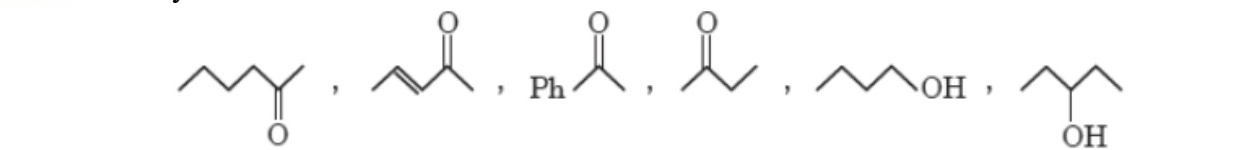
\includegraphics[width=0.72\linewidth]{images_crop_hoa11_de16/tollens_skeletal_structures.png}
\end{center}
Có bao nhiêu chất trong dãy không phản ứng với thuốc thử Tollens?
\vspace{0.8cm}
\end{ex}

\begin{ex}
Cho acetaldehyde và acetone lần lượt tác dụng với thuốc thử Tollens, \ce{Cu(OH)2/NaOH}, HCN, \ce{I2/NaOH}. Có bao nhiêu trường hợp xảy ra phản ứng hóa học?
\vspace{0.8cm}
\end{ex}

\begin{ex}
Cho các hợp chất hữu cơ sau: \ce{CH3CHO}, \ce{(CH3)2CHCHO}, \ce{CH3CH2OH}, \ce{CH3OCH3}, \ce{HCHO}, \ce{CH3COCH2CH3}, $p$-\ce{CH3C6H4CHO}. Có bao nhiêu hợp chất là hợp chất carbonyl?
\vspace{0.8cm}
\end{ex}

\begin{ex}
Cho các hợp chất hữu cơ sau: ethyne, methanol, isopropyl alcohol, acetone, propanal, acrolein, propene, benzene. Có bao nhiêu hợp chất làm mất màu nước bromine ở điều kiện thường?
\vspace{0.8cm}
\end{ex}

\begin{ex}
\textbf{(SBT - CTST)} Acetone được điều chế bằng cách oxi hoá cumene nhờ oxygen, sau đó thuỷ phân trong dung dịch \ce{H2SO4} loãng theo phương trình:
\begin{center}
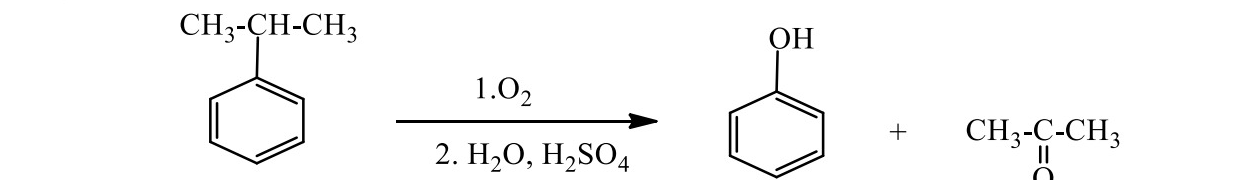
\includegraphics[width=0.72\linewidth]{images_crop_hoa11_de16/cumene_acetone.png}
\end{center}
Để thu được 87 gam acetone thì lượng cumene cần dùng (giả sử hiệu suất quá trình điều chế đạt 80\%) là bao nhiêu gam?
\vspace{0.8cm}
\end{ex}

\bigskip
\noindent\textbf{\large PHẦN IV. Câu hỏi tự luận.}
\textit{Thí sinh trình bày lời giải chi tiết vào giấy làm bài.}
\vspace{0.2cm}

\begin{ex}
\textbf{(SBT - CTST)} Cho sơ đồ phản ứng sau:
\begin{center}
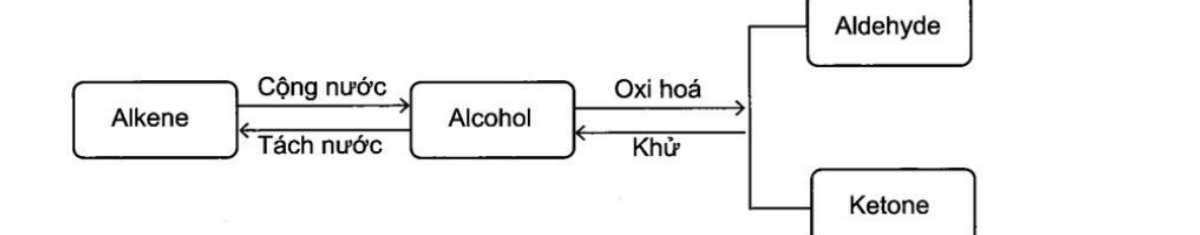
\includegraphics[width=0.68\linewidth]{images_crop_hoa11_de16/alkene_alcohol_carbonyl.png}
\end{center}
Từ alkene ban đầu là \ce{C3H6}, hãy viết các phương trình hóa học tạo ra sản phẩm như sơ đồ trên (kèm điều kiện phản ứng).

\vspace{0.2cm}
\noindent\dotfill\\[4pt]
\noindent\dotfill\\[4pt]
\noindent\dotfill\\[4pt]
\noindent\dotfill\\[4pt]
\noindent\dotfill
\end{ex}

\begin{ex}
Lactic acid hay acid sữa là hợp chất hóa học đóng vai trò quan trọng trong nhiều quá trình sinh hóa, lần đầu tiên được phân tách vào năm 1780 bởi nhà hóa học Thụy Điển Carl Wilhelm Scheele. Lactic acid có công thức phân tử \ce{C3H6O3}, công thức cấu tạo: \ce{CH3-CH(OH)-COOH}. Khi vận động mạnh cơ thể không đủ cung cấp oxygen, thì cơ thể sẽ chuyển hóa glucose thành lactic acid từ các tế bào để cung cấp năng lượng cho cơ thể (lactic acid tạo thành từ quá trình này sẽ gây mỏi cơ) theo phương trình sau:
\begin{center}
\ce{C6H12O6(aq) -> 2C3H6O3(aq)} \quad $\Delta_r H^\circ_{298} = -150\text{ kJ}$
\end{center}
\begin{center}
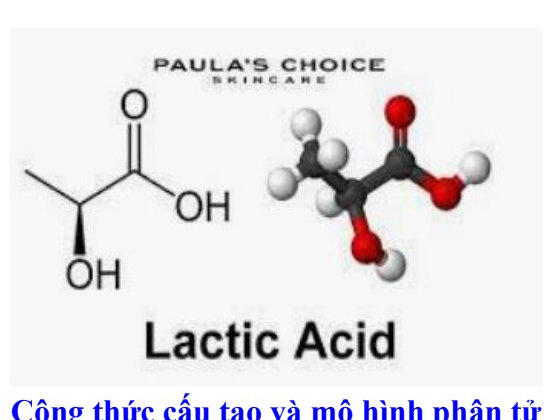
\includegraphics[width=0.45\linewidth]{images_crop_hoa11_de16/lactic_acid_structure.png}
\end{center}
Biết rằng cơ thể chỉ cung cấp 98\% năng lượng nhờ oxygen, năng lượng còn lại nhờ vào sự chuyển hóa glucose thành lactic acid. Giả sử một người chạy bộ trong một thời gian tiêu tốn 300 kcal. Tính khối lượng lactic acid tạo ra từ quá trình chuyển hóa đó (biết $1\text{ cal} = 4,184\text{ J}$).

\vspace{0.2cm}
\noindent\dotfill\\[4pt]
\noindent\dotfill\\[4pt]
\noindent\dotfill\\[4pt]
\noindent\dotfill\\[4pt]
\noindent\dotfill
\end{ex}

\bigskip
\begin{center}
\textbf{---------- HẾT ----------}
\end{center}
\end{document}
